%===================================== CHAP 2 =================================

\chapter{Background Theory}

\section{Artificial Neural Networks}

\textit{This was missing in the specialization project. Need to cover all concepts used later in the report. This includes all different layers of a neural network. The layers (dropout, pooling, etc) could perhaps be a separate section after this one.}

\subsection{The Neuron}

Artificial Neural Networks are inspired by the structure and behavior of a biological brain, although naturally greatly simplified. A neural network consist of interconnected nodes called artificial neurons. These correspond to a biological neuron, the basic computational unit of the brain, illustrated in \textbf{Fig. \ref{fig1}}. The connections between these artificial neurons corresponds to a biological neuron's dendrites, which provide input signals, and its single axon, which produces output signals and is connected to other neurons. \\

\begin{figure}
    \begin{minipage}{0.54\textwidth}
        \centering
            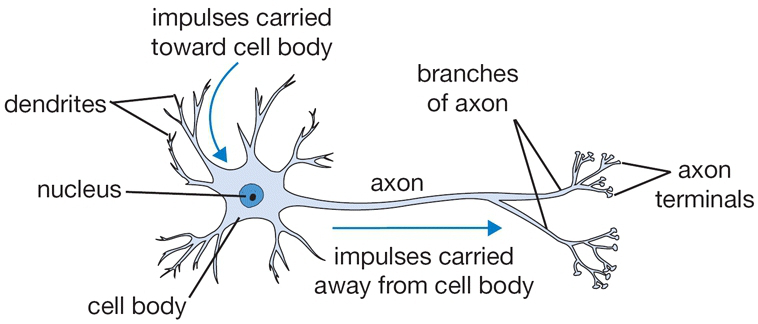
\includegraphics[width=1\textwidth]{fig/neuron}
            \caption{Biological neuron}
            \label{fig1}
    \end{minipage}
    \begin{minipage}{0.4\textwidth}
        \centering
            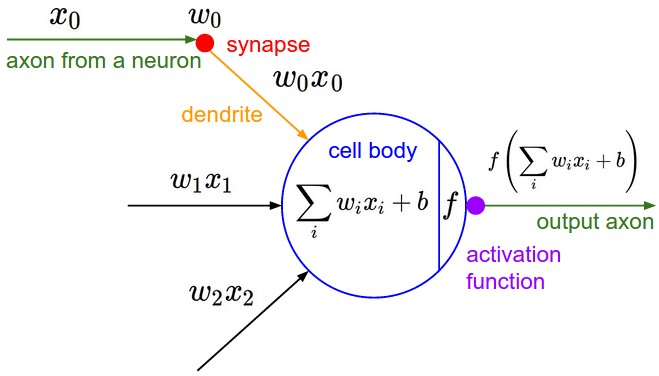
\includegraphics[width=1\textwidth]{fig/neuron_model}
            \caption{Mathematical model}
            \label{fig2}
    \end{minipage}
\end{figure}

\noindent An ANN uses a mathematical model as in \textbf{Fig. \ref{fig2}} to simulate these signals, where the signal is multiplied by the weight of a connection. The weight of a specific connection control how much the neuron on one end influences the neuron on the other end. The sum of all input signals are computed at the cell body of the neuron. If this sum is above a certain threshold, the neuron fires an output signal determined by its activation function. \\

\noindent The weights of a model can be learned by training the model on a set of input and output values. \\

\subsection{The Activation Function}

\begin{itemize}
    \item Sigmoid
    \item Tanh
    \item ReLU
    \item Leaky ReLU
    \item Maxout
\end{itemize}

\subsection{Layers}

\begin{itemize}
    \item Fully-connected layer
\end{itemize}

\section{Convolutional Networks}

\textit{More in-depth than covered in the specialization project. \\
What exactly is the convolutional operation? Convolutional layer (local connections and weight sharing) vs normal layer.}

\section{Residual Networks}

\section{Face Recognition}

\textit{Can probably use a lot from the specialization project here.}

\section{Facial Expression}

\textit{Here as well.}

\section{Visualization}

\textit{Describe all the different techniques, perhaps in more detail. \\
Possibly even implementation level.}

\cleardoublepage